%%%%%%%%%%%%%%%%%%%%%%%%%%%%%%%%%%%%%%%%%%%%%%%%%%%%%%%%%%%%%%%%%%%
%                                                                 %
%                            APPENDICES                           %
%                                                                 %
%%%%%%%%%%%%%%%%%%%%%%%%%%%%%%%%%%%%%%%%%%%%%%%%%%%%%%%%%%%%%%%%%%%
 
\appendix    % This command is used only once!
%\addcontentsline{toc}{chapter}{APPENDICES}             %toc entry  or:
\addtocontents{toc}{\parindent0pt\vskip12pt APPENDICES} %toc entry, no page #
\let\cleardoublepage\clearpage
\chapter{YouBot driver}
\label{sec:appendixA}
The youBot base or the manipulator can be controlled in three different modes as discussed in the introduction section. The interface details~\cite{youbotdriver}~\cite{youbotdriver_architecture} of the driver that are used in this project are briefed in this section. It is important to obtain the handle reference for the youBot manipulator or the base in order to command the data or retrieve the sensed data from the joints. The handle to the youBot manipulator can be obtained by creating an object to the following class

\begin{verbatim}
youbot::YouBotManipulator *youbotArm(Arm_name, Path_to_config_directory);
\end{verbatim}

and the handle for the youBot base can be obtained similarly

\begin{verbatim}
youbot::YouBotBase *youbotBase(Base_name, Path_to_config_directory);
\end{verbatim}

This work explains only the implementation details of the youBot manipulator and the youBot base can also be controlled in the similar way. The robot joints can be controlled individually or collectively. The position/velocity/torque commands to the joints has to be prepared and can be given as follows

\begin{verbatim}
vector<youbot::JointAngleSetpoint> jointAngleCommands(Total_Joints);
vector<youbot::JointVelocitySetpoint> jointVelocityCommands(Total_Joints);
vector<youbot::JointTorqueSetpoint> jointTorqueCommands(Total_Joints);
\end{verbatim}

where Total\_Joints represents the number of joints in the manipulator. The measured joint information for all the joints can be read with the use of the following classes

\begin{verbatim}
vector<youbot::JointSensedAngle> jointAnglesMeasured(Total_Joints);
vector<youbot::JointSensedVelocity> jointVelocitiesMeasured(Total_Joints);
vector<youbot::JointSensedTorque> jointTorquesMeasured(Total_Joints);
\end{verbatim}

With the use of the above classes, it is now possible to set or get the angle (in radians) for all the joints of manipulator with the use of the following methods

\begin{verbatim}
youBotArm->setJointData(jointAngleCommands);
youBotArm->getJointData(jointAnglesMeasured);
\end{verbatim}

The velocity, torque modes can also be controlled similarly with the use of the above given methods. 

\chapter{Orocos KDL}
\label{sec:appendixB}

At first the kinematic chain of the youBot manipulator has to be created as follows

\begin{verbatim}
KDL::Chain kinematicChain;
\end{verbatim}

The manipulator is represented by the kinematic chain of rigid bodies or segments. The next step is to add the segments of the manipulator to the kinematic chain that has been created in the previous step. 

The segments can be created by instantiating an object to the following class

\begin{verbatim}
KDL::Segment segment(name, joint_axis, frame, rigid_body_inertia);
\end{verbatim}

where the segment defines both the joint information and link properties which are then added to the chain by using the following method

\begin{verbatim}
kinematicChain.addSegment(segment);
\end{verbatim} 

Once the complete kinematic chain of the manipulator is created, the kinematics and dynamics of kinematic chains can be computed. The Orocos KDL library provide solvers for both the forward and inverse kinematics computations. This work made use of the forward kinematics solver to find the end-effector's pose and the solver can be instantiated and invoked as given below.

\begin{verbatim}
KDL::ChainFkSolverPos_recursive::JntToCart(q, T)
\end{verbatim} 

where q represents the joint position inputs for the manipulator joints and T represents the frame (KDL::Frame) that gives the pose information of the end-effector. The dynamics of the kinematic chain can be computed by using the recursive Newton-Euler formulation which is implemented based on the article~\cite{featherstone2014rigid}. Though the semantics used is same as the article, there is an important difference in the semantics of the algorithm in KDL comparing the article, i.e. In ~\cite{featherstone2014rigid}, author uses the spatial vector transforms in the algorithm whereas KDL does not uses the spatial form. The ID solver which is used in KDL can be invoked as follows

\begin{verbatim}
KDL::ChainIdSolver_RNE idsolver;
idsolver.CartToJnt(position, velocity, acceleration, wrench, torques);
\end{verbatim}

\chapter{Simbody}
\label{sec:appendixC}

At first the visualizer has to be created with the use of the class SimTK::Visualizer where the properties can be adjusted based on the system needs and an event reporter (PeriodicEventReporter) is attached to handle the events of the system at the defined intervals. The time stepper (SimTK::TimeStepper) uses SimTK::RungeKuttaMersonIntegrator to take the system forward through time. The system is initialized after the system model is created. The forces can be commanded to the manipulator joints as generalized forces by using the class SimTK::GeneralForceSubSystem. The more detailed reference can be found in\footnote{\url{https://simtk.org/api_docs/simbody/3.5/namespaceSimTK.html}} and the implementation details are specified as follows. In Simbody, the multi-body system is created at first and the sub-systems are attached for the further operations. The system has a subclass SimTK::MultibodySystem to work with the general multi-body systems along with the sub-system SimTK::SimbodyMatterSubSystem which is responsible for defining all the rigid bodies in the system. 

\begin{verbatim}
SimTK::MultibodySystem system;
SimTK::SimbodyMatterSubSystem matterSubSystem(system);
\end{verbatim}

The gravity can be simulated with the use of the following class

\begin{verbatim}
SimTK::Force::Gravity gravity = SimTK::Force::Gravity();
\end{verbatim}

A rigid body can be created and the link properties can be attached with the help of the following classes

\begin{verbatim}
SimTK::Body rigid_body;
rigid_body = SimTK::Body::Rigid(SimTK::MassProperties(mass, CoM, Inertia));
\end{verbatim}

The joints can be created with the use of the MobilizedBody class

\begin{verbatim}
SimTK::MobilizedBody body(Number_of_joints);
\end{verbatim}

Before attaching the rigid bodies to the sub-system, it is important to attach the base body to the ground (parent body) which is the origin by using the weld joint

\begin{verbatim}
body = SimTK::MobilizedBody::Weld();
\end{verbatim}

The revolute joints can be attached to the mobilized body with the help of the Pin  class which attaches a new body to the system with the one DoF constraint to the predecessor.

\begin{verbatim}
body = SimTK::MobilizedBody::Pin();
\end{verbatim}

The joint information such as position, velocity and acceleration are retrieved from the state of the system that gets updated in a periodic manner. The torque sensor has been created in this work with the use of the SimTK interface that measures the gravitational, bias and the custom forces from the multi body system. It is possible to command the generalized coordinate with the particular motion as a function which can be step or sinusoid use of the following class

\begin{verbatim}
SimTK::Constraint::PrescribedMotion
\end{verbatim}

The two-link manipulator has been created to test the prescribed motion in this work to verify the semantic correctness and setting the joint positions required the update in the state variable which is a constant in Simbody and the setup for the 2-link manipulator is depicted in Fig.~\ref{fig:simbody_2link}.

\begin{figure}[H]
\centering
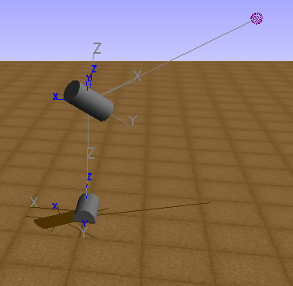
\includegraphics[width=50mm, trim=0 0 0 0]{pictures/simbody_2link_manipulator}
\caption{Two-link manipulator is constructed with the cylinder objects in Simbody visualizer for commanding the prescribed motion to the mobilizer}
\label{fig:simbody_2link}
\end{figure}

\chapter{Tuning of the controller gains}
\label{sec:appendixD}

\begin{figure}[H]
\centering     %%% not \center
\subfigure[Inner loop tuning]{\label{fig:joint5_innerloop_1rads}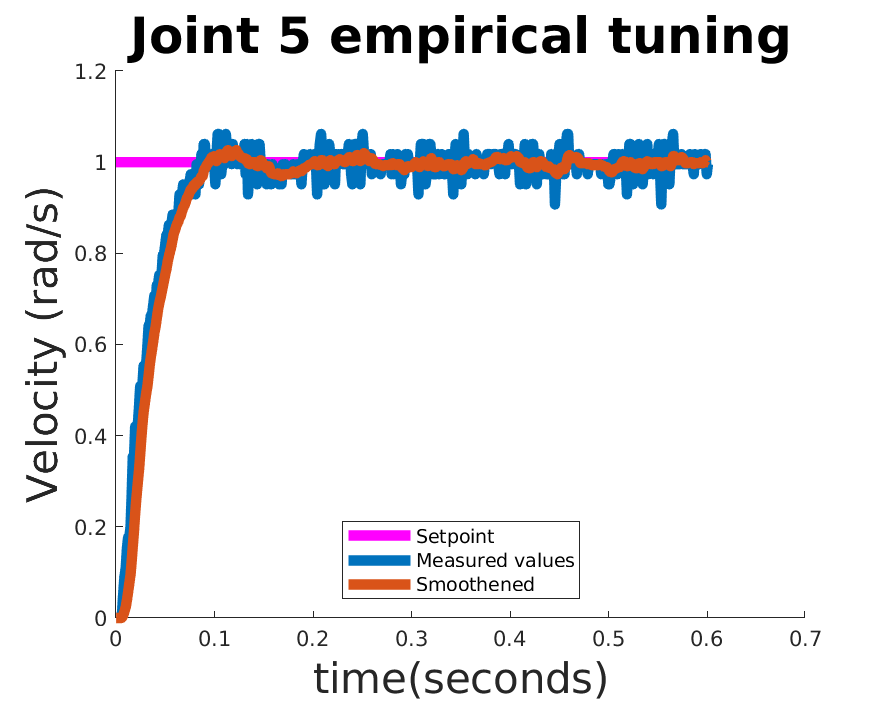
\includegraphics[width=70mm]{pictures/joint5_innerloop_1rads}}
\subfigure[Outerloop tuning]{\label{fig:joint5_outerloop_1rad}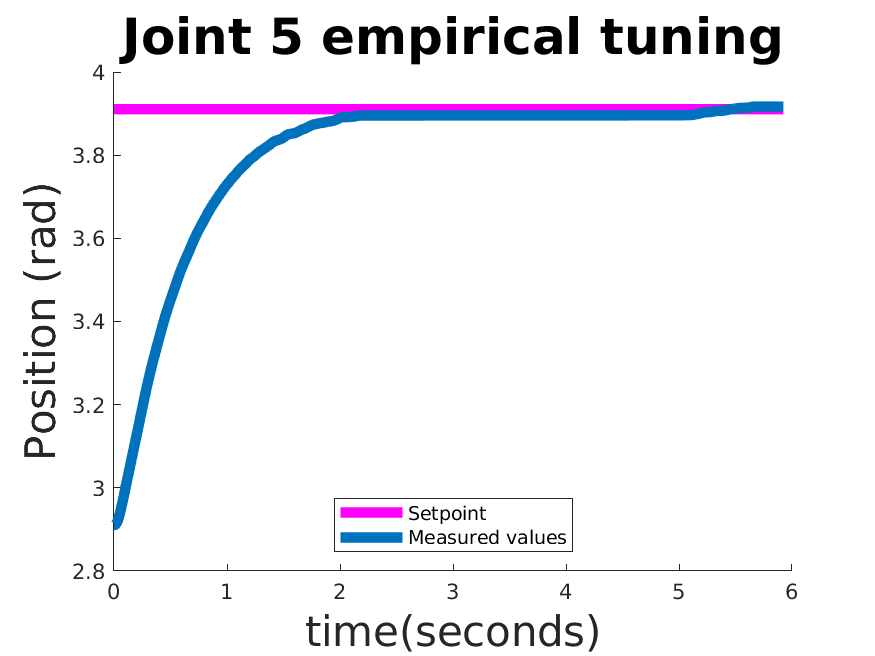
\includegraphics[width=70mm]{pictures/joint5_outerloop_1rad}}
\caption{Inner, outer loop tuning for joint 5 with the velocity, position set-points of 1.0 rad/s, 1.0 rad respectively}
\end{figure}

\begin{figure}[H]
\centering     %%% not \center
\subfigure[Inner loop tuning]{\label{fig:joint5_innerloop_1pt5rads}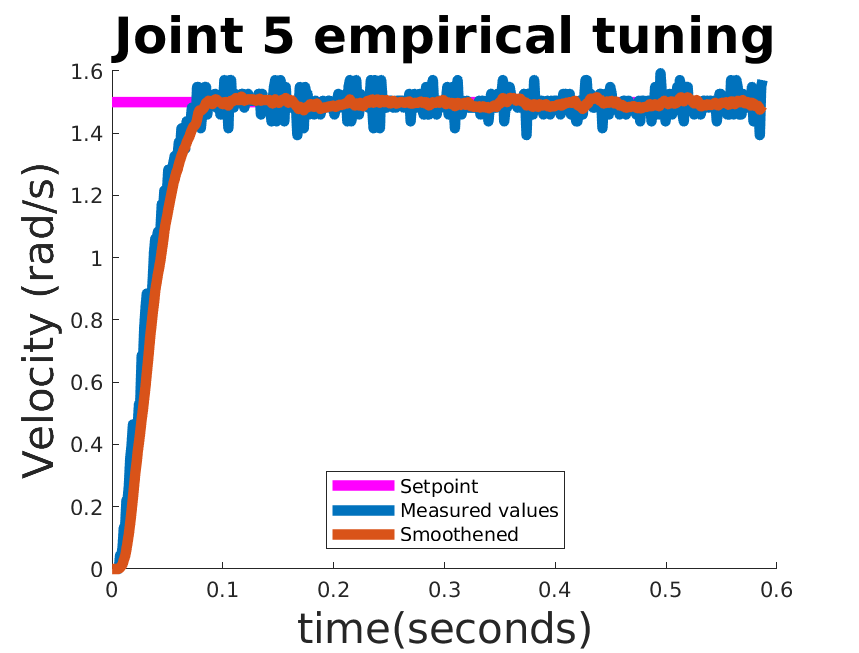
\includegraphics[width=70mm]{pictures/joint5_innerloop_1pt5rads}}
\subfigure[Outerloop tuning]{\label{fig:joint5_outerloop_1pt5rad}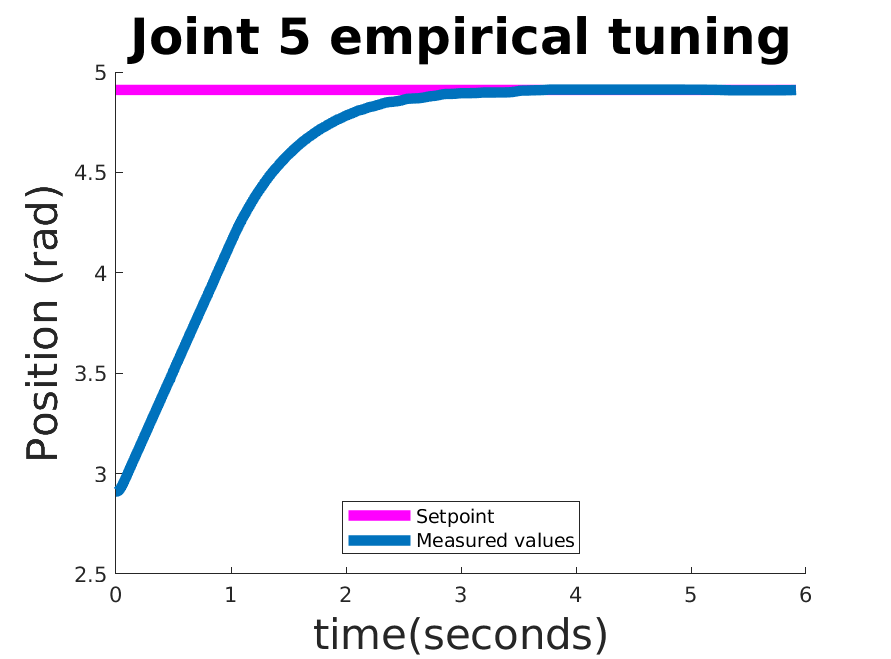
\includegraphics[width=70mm]{pictures/joint5_outerloop_2rad}}
\caption{Inner, outer loop tuning for joint 5 with the velocity, position set-points of 1.5 rad/s, 1.0 rad respectively}
\end{figure}

